\section{Attention and Transformers}
\subsection{Sequence-to-sequence with RNNs and attention}
\subsubsection{Encoder-decoder RNNs and limitations}
Originally, the transformer architecture was proposed for machine translation, and was later extended to other deep learning domains. To introduce the attention mechanism, let's consider a machine translation setup; we will start by building up on top of the RNN architecture introduced in the previous chapter.

We are given a sentence in English and want to translate it in French. To do so, we use two RNNs, an encoder which will handling the input tokens, and a decoder which will generate the output sentence.
\begin{figure}[H]
    \centering
    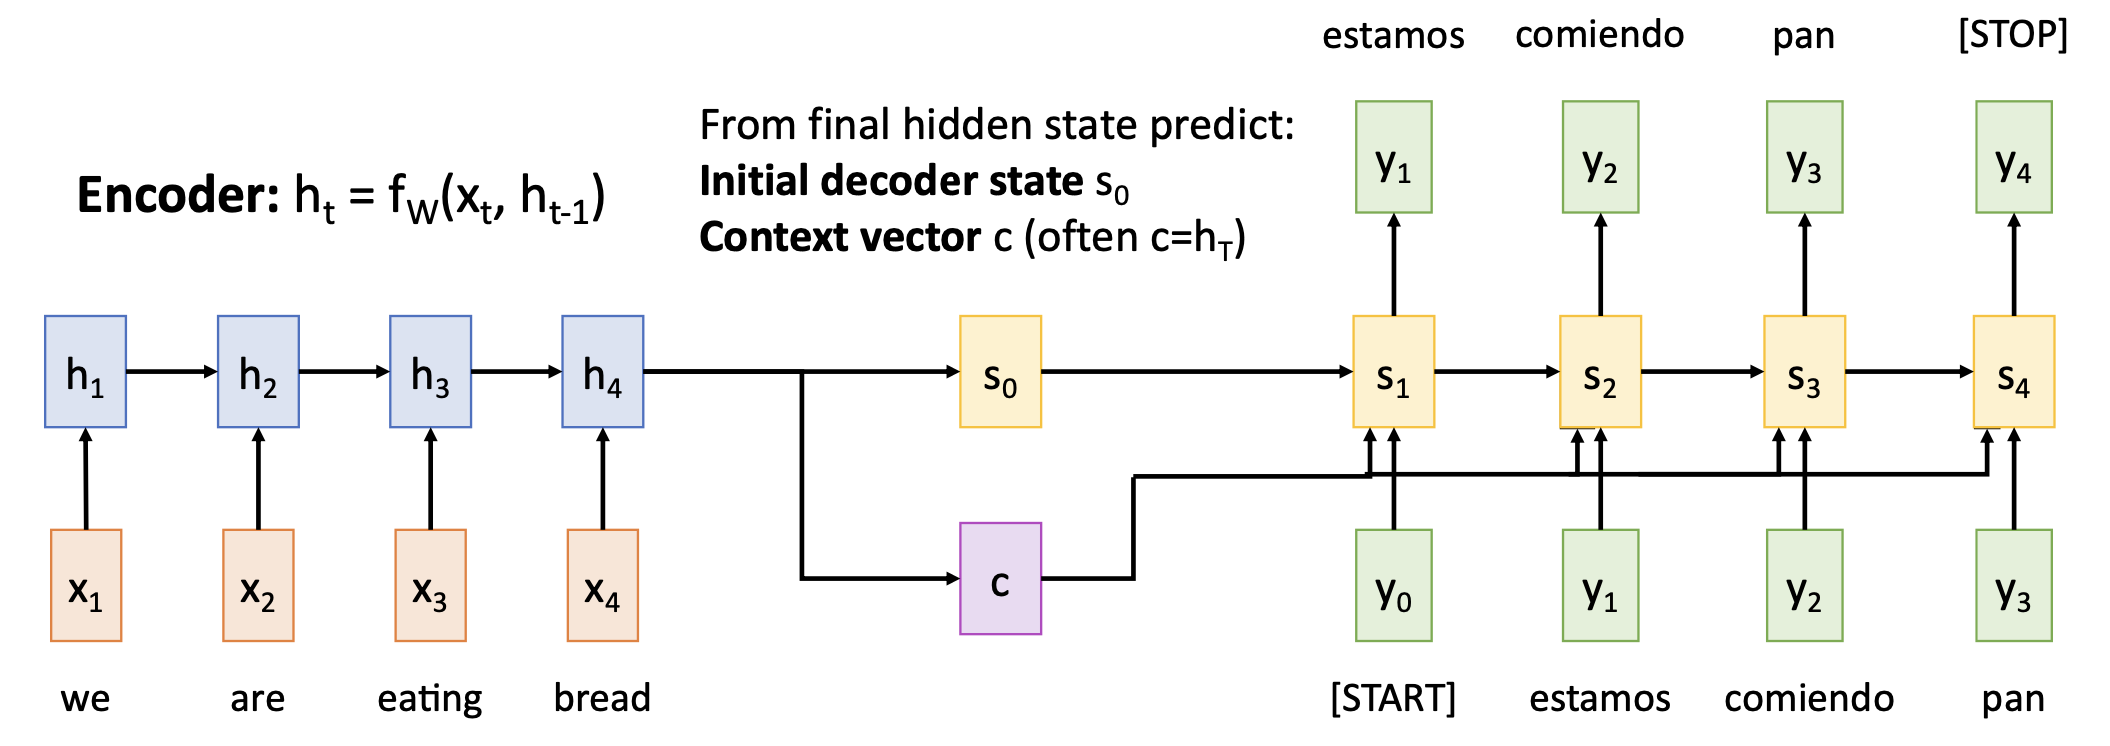
\includegraphics[width=\textwidth]{images/seq-to-seq.png}
    \caption{Sequence-to-sequence using an RNN.}
\end{figure}
After the processing of the original sentence, the encoder will summarize the entire context of that input sentence using two vectors: the initial decoder state $s_0$, and the context vector $c$. In practice, $s_0$ is often obtained by feeding $h_T$ through a feed-forward neural network, and $c$ is often set to $h_T$ directly.

The decoder will receive a start token $y_0$ as its first input, as well as the context vector $c$; it will then generate the first output token $y_1$, which will be used as the second input. Note that the context $c$ is fed to the decoder at each step of the generation, on top of the last generated token $y_t$. Formally, its recurring equation is of the form:
\begin{equation*}
    s_t = g_{W'}(y_{t-1}, s_{t-1}, c)
\end{equation*}

While this architecture is fairly reasonable, its bottleneck is that the entire context of the sentence must be summarized in the fixed-size context vector $c$. If the text to translate is too long (think of an entire book for instance), the model will not be able to fit all the context details in $c$. The idea to solve this issue is to compute a new context vector at each step of the decoder, and to allow the decoder to reconstruct the context vector by using different vectors focusing on different parts of the original sentence. This mechanism is called \emph{attention}.

\subsubsection{The attention mechanism}
We will keep the general encoder-decoder structure, but instead change the way that the context is passed from the encoder to the decoder. We will use an MLP called $f_{\textnormal{att}}$, which will compute scalar alignment scores:
\begin{equation*}
    e_{t,i} = f_{\textnormal{att}}(s_{t-1}, h_i)
\end{equation*}
Intuitively, the alignment score $e_{t,i}\in\R$ quantifies how much \emph{attention} should be put in the hidden state of the encoder $h_i$, given the hidden state of the decoder $s_{t-1}$. These scalars will be used to construct a new context vector at each step of the decoder.

\begin{figure}[H]
    \centering
    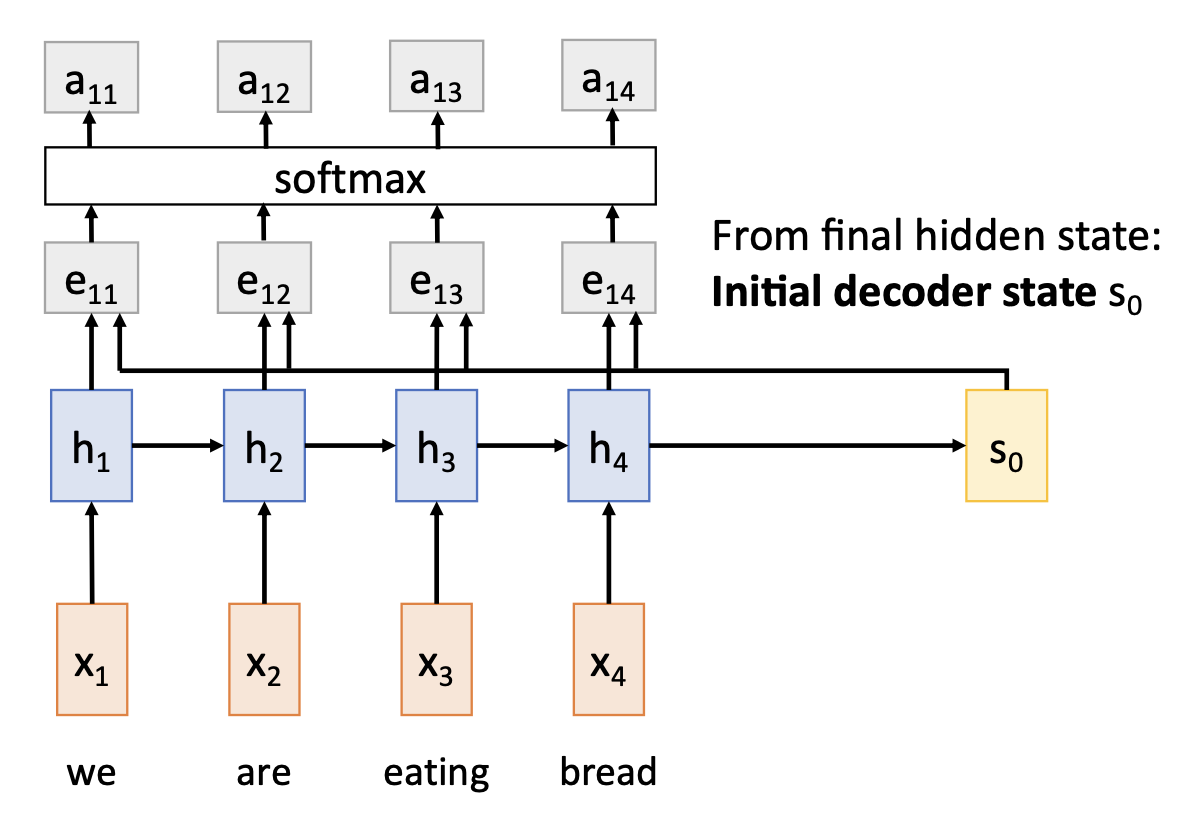
\includegraphics[width=.5\textwidth]{images/attention-scores.png}
    \caption{Applying softmax to alignment scores gives us attention scores.}
\end{figure}

The alignment scores are arbitrary real numbers. Therefore, we apply to them the softmax operations for each decoder state $s_{t-1}$, giving us \emph{attention weights} $(a_{t,i})$ satisfying:
\begin{equation*}
    \sum_i a_{t,i} = 1 
\end{equation*}
That being done, we can finally compute the context vector for each time step $t$ of the decoder, using a sum of the hidden states $(h_i)$ weighted by the attention scores $(a_{t,i})$:
\begin{equation*}
    c_t = \sum_i a_{t,i}\cdot h_i
\end{equation*}
This gives us the context vector $c_t$ which will be used for the generation of $y_t$ by the decoder. Note that this is all differentiable and allows us to backpropagate through the parameters of $f_{\textnormal{att}}$; in particular, we do not need to supervise the attention weights.
\begin{figure}[H]
    \centering
    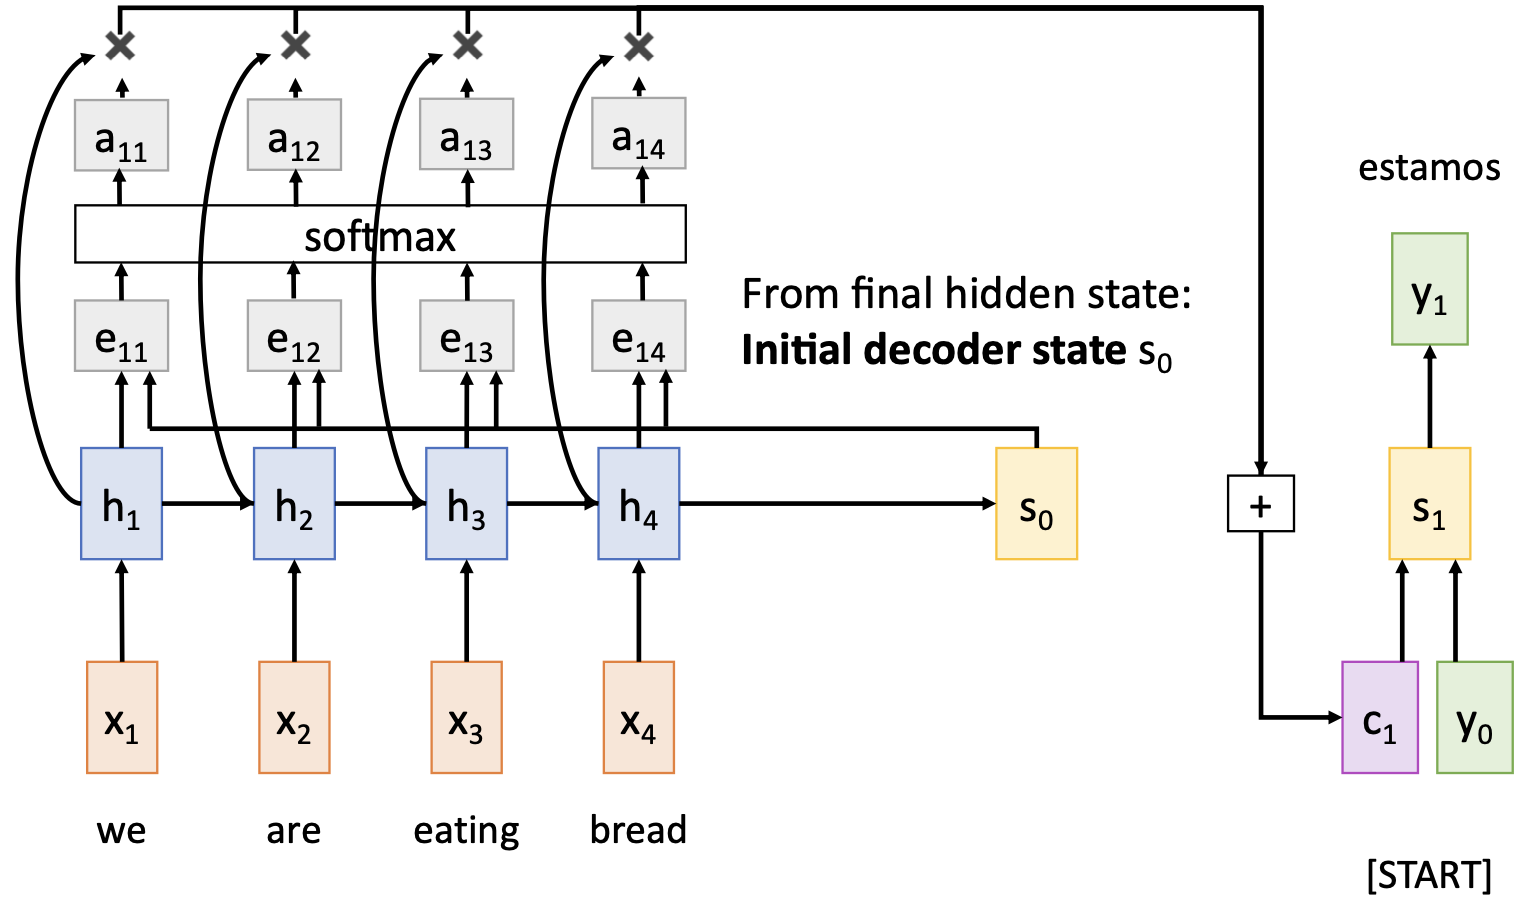
\includegraphics[width=.65\textwidth]{images/attention-context.png}
    \caption{Computation of the context vector using attention scores.}
\end{figure}
This process that was applied for the first decoder step $t=1$ can be iterated for every following step: we compute the alignment scores using the new hidden state $s_1$, then the attention scores, giving us the context vector $c_t$, which is fed into the decoder alongside $y_{t-1}$.
\begin{figure}[H]
    \centering
    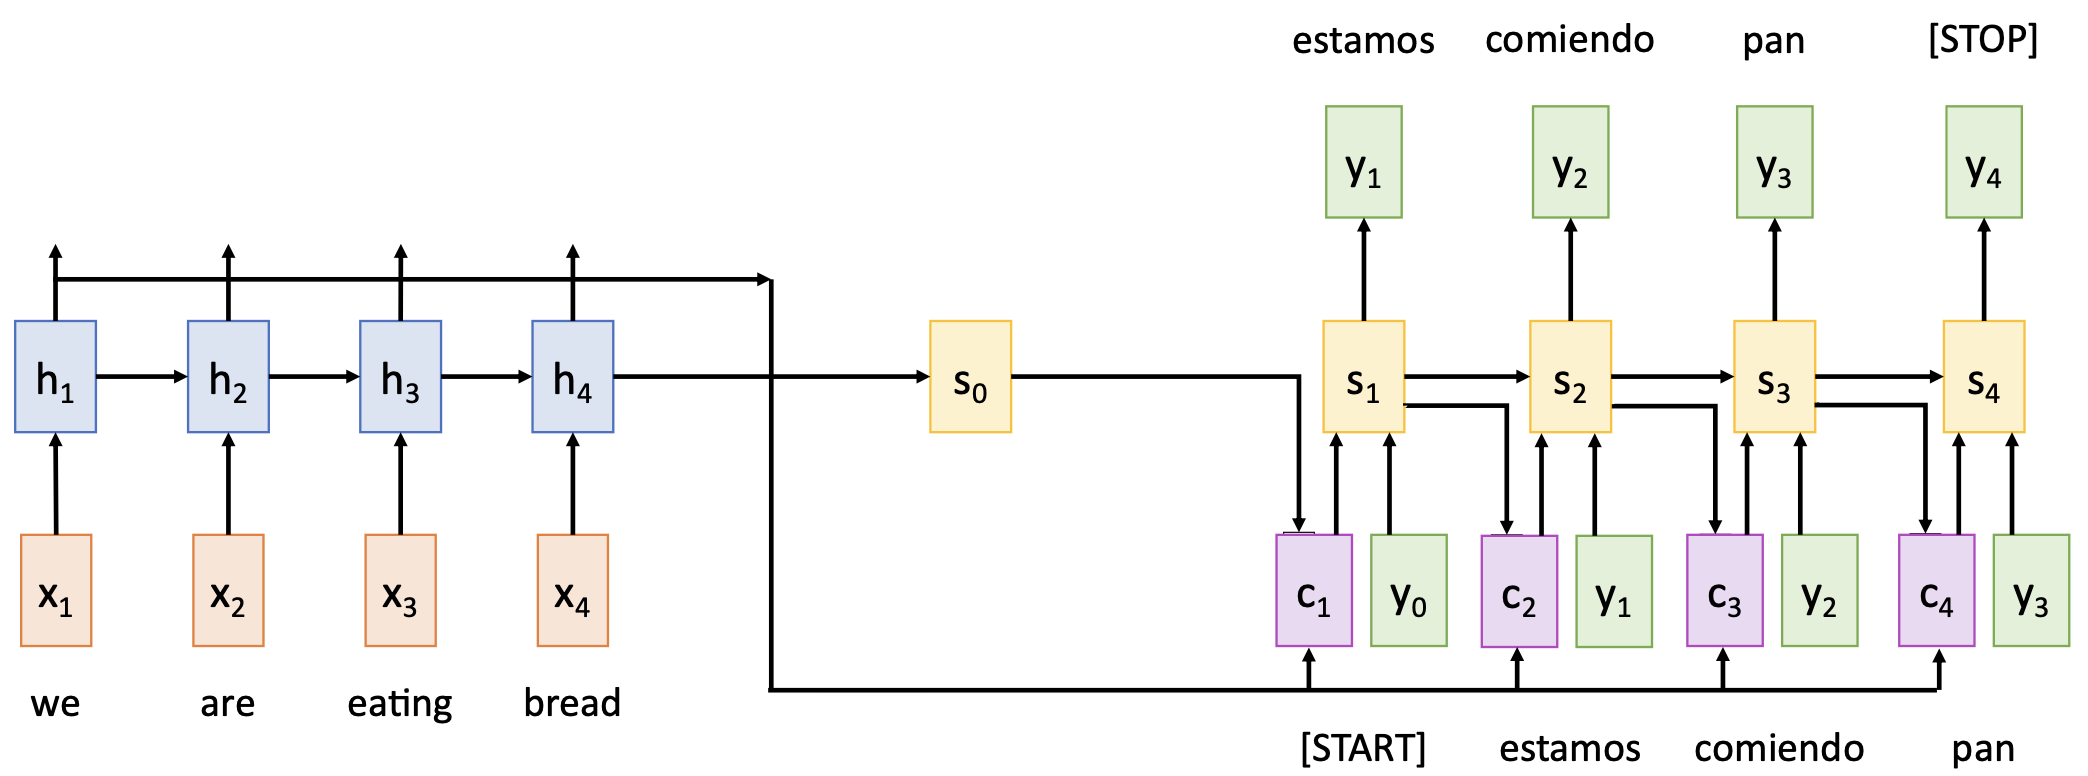
\includegraphics[width=.9\textwidth]{images/attention-unrolled.png}
    \caption{Unrolling the computational graph with attention.}
\end{figure}
This overcomes the bottleneck problem encountered for unique context vectors: at each step, the decoder is able to choose the relevant hidden states of the encoder, which selects only relevant information. When working with very long sequences, the model will be able to shift its attention around and focus on important parts of the inputs.

\subsection{Visualizing and interpreting attention weights}
\begin{wrapfigure}[14]{r}{.45\textwidth}
    \captionsetup{justification=raggedleft}
    \centering
    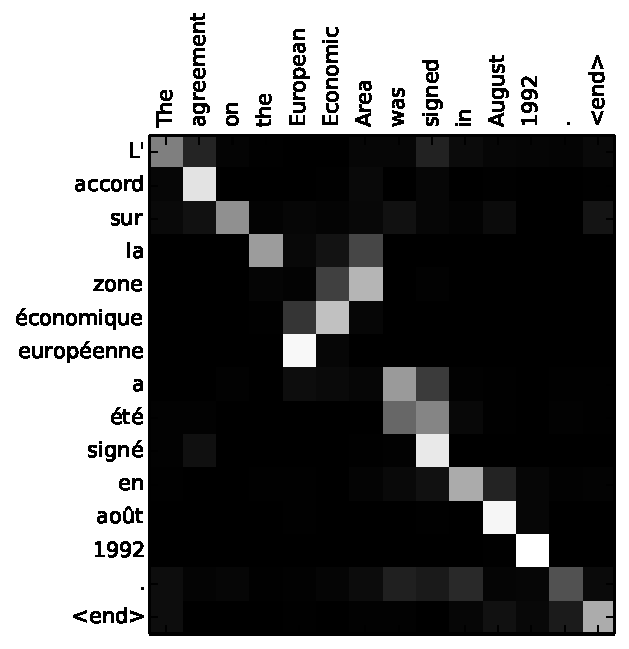
\includegraphics[width=.45\textwidth]{images/attention-visualization.pdf}
    \caption{Visualization of attention weights for English-to-French translation.\protect\footnotemark}
\end{wrapfigure}
\footnotetext{Image taken from Bahdanau et al, \say{Neural machine translation by jointly learning to align and translate}, ICLR 2015}
The attention weights can be used to gain interpretability of the model: we can see for each output word which original words it was the most focused on.  

Diagonal attention (the first four words and the last 5 words) means that words correspond in order between French and English. High coefficients outside the diagonal (for instance, \say{European}/\say{européenne}) show words out of order between the two sentences. Finally, some lines and columns have more than one non-zero coefficient, such as the \say{was} or \say{say} columns: these show that the verb conjugation requires more than one word of context to be translated.

\newpage
\subsection{Image captioning with RNNs and Attention}
It is important to notice that the decoder does not use the fact that the hidden states $(h_i)_i$ form an ordered sequence, but only considers them as an unordered set $\set{h_i}{i\in I}$. This means that we can use the same architecture given any set of input hidden vectors $\set{h_i}{i\in I}$, especially for other types of data that do not form sequences.

Consider a deep convolutional neural network, without fully-connected layers at the end. The ouput of this CNN can be interpreted as a grid of feature vectors of the image. We see these feature vectors just like a sequence of hidden states of an encoder RNN: we can therefore apply the attention mechanism to them. We consider a simple model $f_{\textnormal{acc}}$ that we use to compute the alignment scores of each feature in the grid:
\begin{equation*}
    e_{t,i,j} = f_{\textnormal{att}}(s_{t-1}, h_{i,j})
\end{equation*}
We then pass each grid of alignment scores into the softmax operator, giving us a normalized probability distribution, the grid of attention weights $(a_{t,i,j})$. Once again, the context of the image can be summarized with respect to the attention weights by computing a context vector $c_t$:
\begin{equation*}
    c_t = \sum_{i,j} a_{t,i,j} \cdot h_{i,j}
\end{equation*} 
Feeding the context vector $c_1$ alongside the start token $y_0$ into the decoder RNN starting with hidden state $s_0$ can be used to generate a caption corresponding to the image.
\begin{figure}[H]
    \centering
    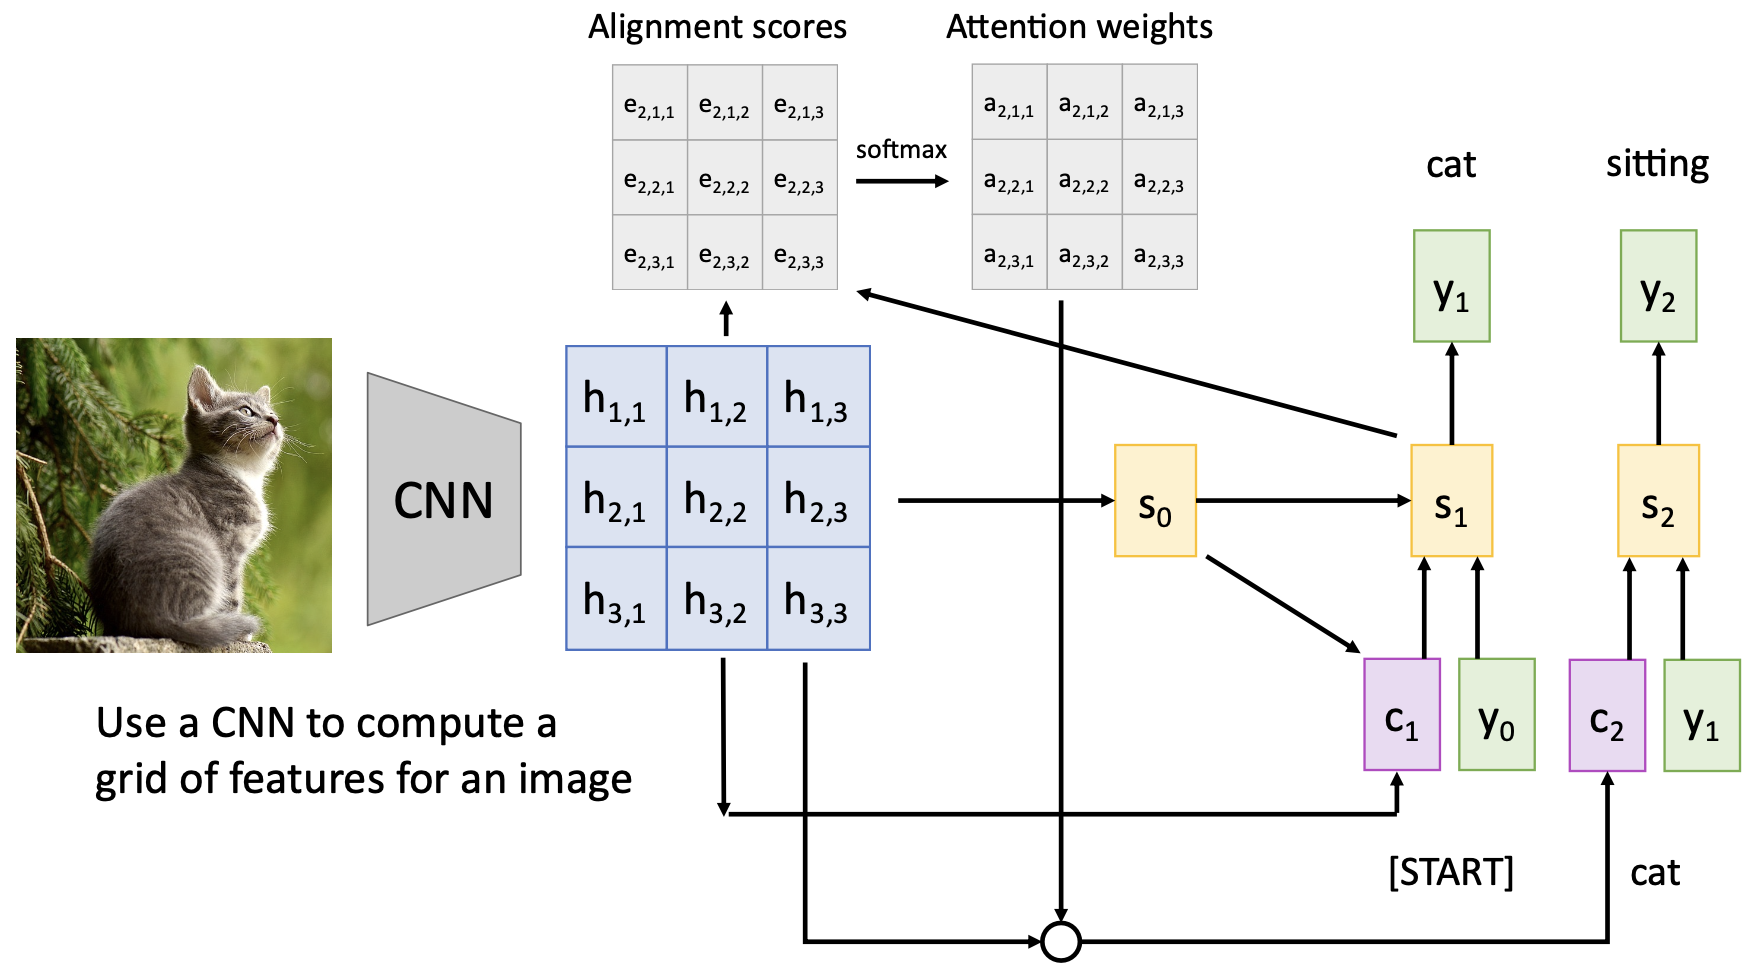
\includegraphics[width=.9\textwidth]{images/attention-cnn.png}
    \caption{Applying attention to a grid of features for image captioning.}
\end{figure}

\begin{figure}[H]
    \centering
    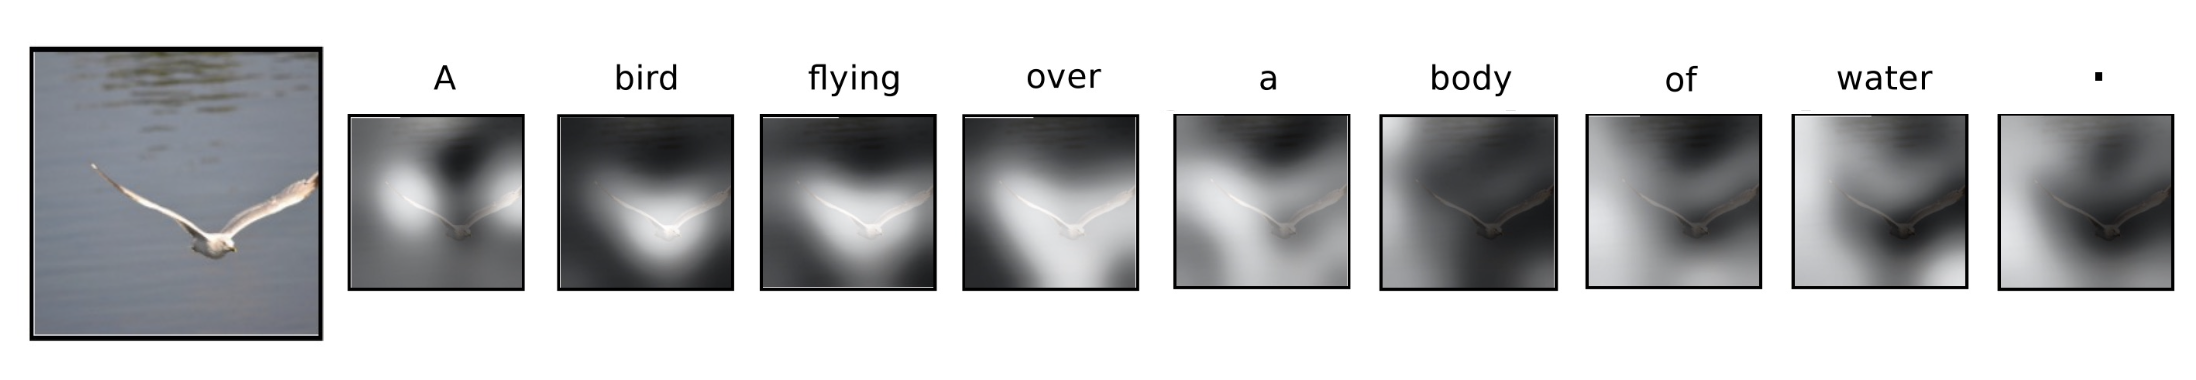
\includegraphics[width=\textwidth]{images/attention-bird.png}
    \caption{Visualizing attention over time during captioning.\protect\footnotemark}
\end{figure}
\footnotetext{Image taken from Xu et al, \say{Show, Attend, and Tell: Neural Image Caption Generation with Visual Attention}, ICML 2015}

\newpage